\subsection{Objective 1: \texttt{mpbenchmark}}
As mentioned in the introduction section \texttt{mpbenchmark} performs calculations of a jet engine using multiple threads and produces the time taken to complete these calculations as output. After analysing the code implementation of \texttt{mpbenchmark} the application can be summarised performing the following tasks:

\begin{enumerate}
	\item The application reads data from an input(\texttt{.txt}) file and stores that into an array before starting the calculations. This input data is required to perform calculations required in the next step. 
	\item During calculation, each thread reads input data at specific positions of the input array. After calculation, the results are written into an output array.
	\item In the last step, the benchmark’s response time along with deadlines missed is printed out and saved to an output(\texttt{.txt}) file. 
\end{enumerate}

This design of \texttt{mpbenchmark} can be visualised in figure \ref*{fig:revised_mpbenchmark_structure}.

\begin{figure}[h] % Positioning preference: here, top, bottom, page
	\centering
	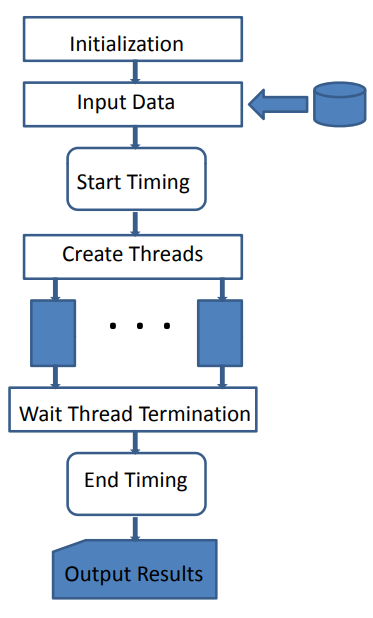
\includegraphics[width=0.5\textwidth, height=10cm]{~/Documents/Part_D_Modules/Individual_Project/Individual_report/figures/revised_mpbenchmark_structure.png} % Adjust the path and width as needed
	\caption{Revised \texttt{mpbenchmark} structure \cite{mpbenchmark_paper}.}
	\label{fig:revised_mpbenchmark_structure} % Use this label to reference the figure
\end{figure}

The source code of \texttt{mpbenchmark} provided a solution in \texttt{C\#}, this served as a useful reference of how figure \ref*{fig:revised_mpbenchmark_structure} would be implemented in code using object-oriented design. Subsequently, the \texttt{C++} object oriented design comprised of three main classes:

\begin{enumerate}
	\item \texttt{FileDataLoader}: the primary function of this class is to load data from the input file and also to allow the user to save output data to the output file.
	\item \texttt{SharedPerformanceData}: this class stores data loaded from the input file into an array and also allows storage of output data into a separate array. But importantly it allows threads to access specific parts of the input data in a thread-safe manner. 
	\item \texttt{Worker}: this class contains functions to perform the important calculations, computations of deadlines missed and output data. This class defines the \texttt{operator ()} which encapsulates the main calculations, this class design is know as a \texttt{Functor}.
\end{enumerate}

The \texttt{C++} object-oriented class design can be visualised using a UML class diagram shown in figure \ref*{fig:mpbenchmark_UML_diagram}.

\begin{figure}[h] % Positioning preference: here, top, bottom, page
	\centering
	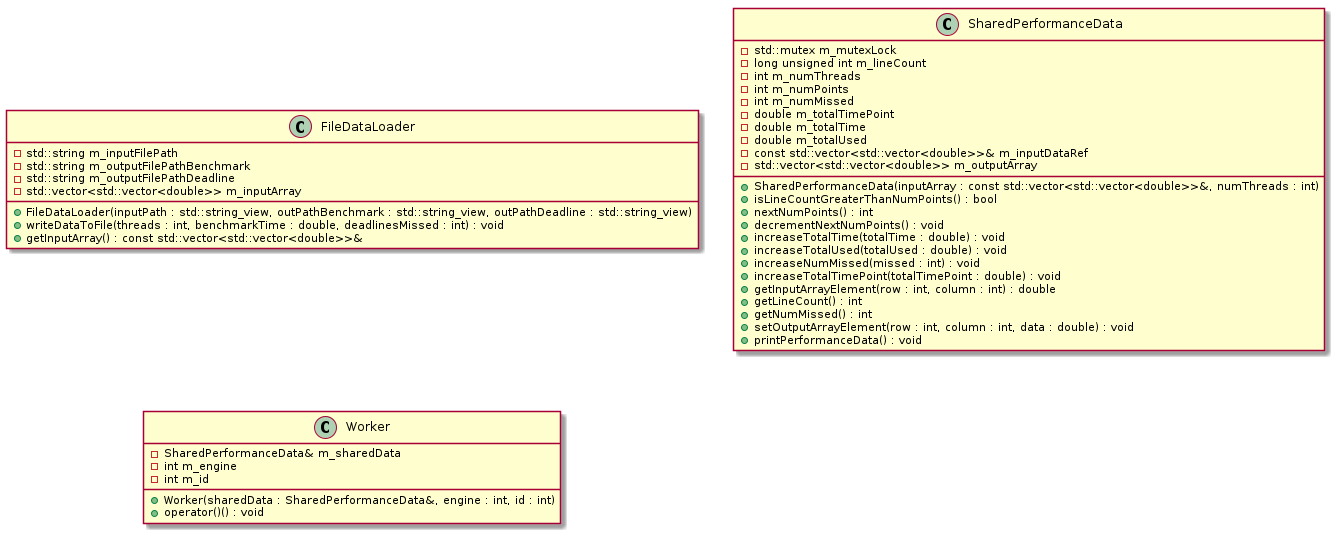
\includegraphics[width=1\textwidth, height=60cm]{~/Documents/Part_D_Modules/Individual_Project/Individual_report/figures/mpbenchmark_class.png} % Adjust the path and width as needed
	\caption{UML class diagram of the proposed \texttt{C++} solution.}
	\label{fig:mpbenchmark_UML_diagram} % Use this label to reference the figure
\end{figure}

These classes are used in the following sequence in the proposed solution[insert UML sequence diagram]:

The \texttt{mpbenchmark} implementation in the \texttt{C} language used \texttt{printf} function for printing throughout the application. Porting this printing functionality to C++ was a slight challenge as \texttt{printf} uses format string based formatting compared to the stream-based formatting used by \texttt{std::cout} in \texttt{C++}. This limitation in \texttt{C++} was addressed in \texttt{C++20} standard by the use of \texttt{std::format}, strangely \texttt{std::format} was not available on the \texttt{gcc} compiler version on target system despite the compiler supporting \texttt{C++20} standard[insert reference]. A work around for this problem was to use the \texttt{fmt::print} function from the \texttt{fmt} library in \texttt{C++}, this library has been reported as being the inspiration for the \texttt{std::format} functionality[insert reference] . Full system specifications and code snippet regarding the usage of fmt::print can be found in the appendix. 

The original \texttt{mpbenchmark} code featured a command line argument that enabled the user (or developer) to specify the engine type for performing calculations. The application supports three different engine types. Crucially, the number of threads utilized by the application could be adjusted using the \texttt{taskset} command in \texttt{Linux}, which specifies the CPU cores that the application is permitted to run on. To enhance functionality, a second command line argument was introduced in the proposed solution. This new argument allows the user to specify the desired number of threads for the application to use. If this parameter is left unspecified, the application defaults to utilizing the maximum number of threads available on the system. This enhancement is illustrated in the following code snippet(listing \label{lst:main})[move to appendix]:

\begin{lstlisting}[
	caption={Command line arguments of the new \texttt{mpbenchmark} solution.},
	label={lst:main_file_cpp}
	]
	int main(int argc, char *argv[]){
		int engine{};
		int numThreads{};
		
		if (argc > 1) {
			engine = std::atoi(argv[1]); // Convert the argument to an integer
		}
		
		if (argc > 2) {
			numThreads = std::atoi(argv[2]); // Convert the argument to an integer
		}
		
		// If the number of threads is not specified, default to the maximum available
		if (numThreads == 0) {
			numThreads = std::thread::hardware_concurrency();
		}
		
		// ignore the other remaining code...
	}
\end{lstlisting}


To compile and link the application, the industry standard \texttt{CMake}[insert citation] software was used. In the \texttt{CMakeLists.txt}(the file used for building the project), the key aspects were specifying the \texttt{C++20} standard, including the \texttt{fmt} library and compilation with the \texttt{-O2} flag. This compilation flag was also used by the authors of \texttt{mpbenchmark}\cite{mpbenchmark_paper} therefore it was used in the proposed solution for consistency. 

\subsection{Objective 2: \texttt{MobileNet}}
\subsection{Objective 3: \texttt{Debate-FI platform}}